\documentclass[tikz]{standalone}

\usepackage{pgfplots}
\pgfplotsset{compat=1.16}

\begin{document}
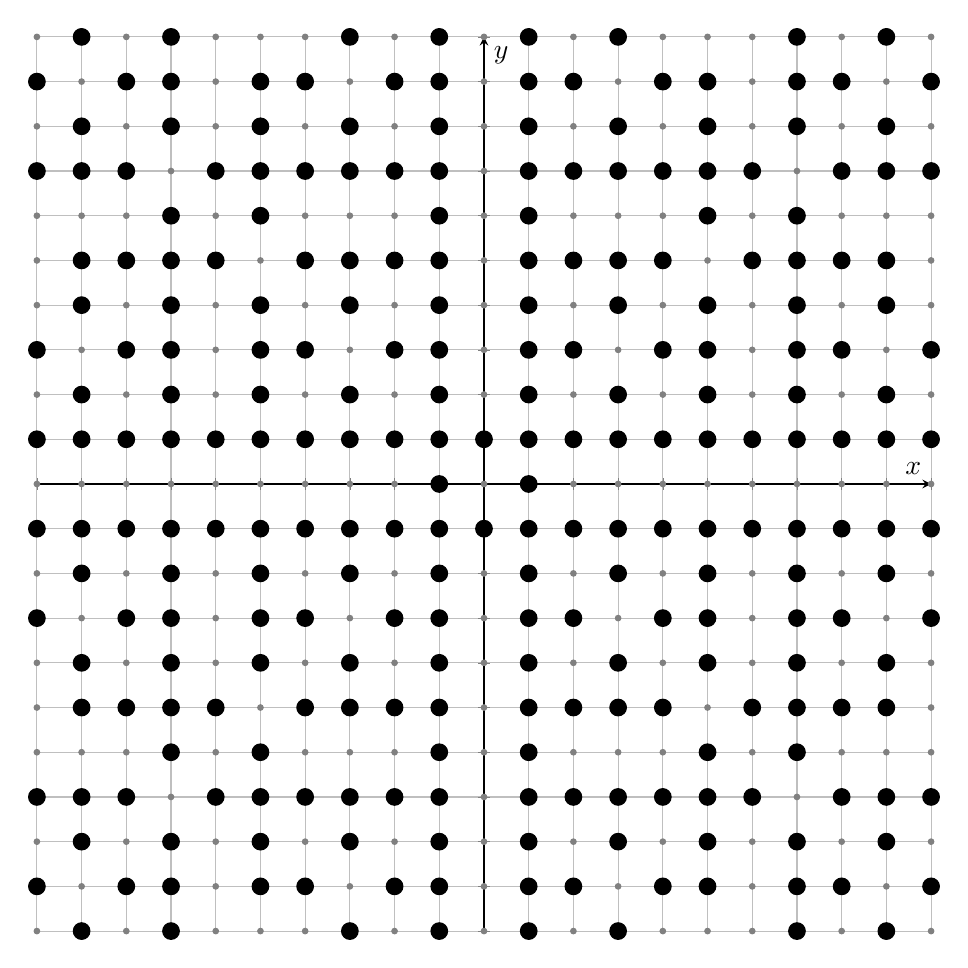
\begin{tikzpicture}
    \begin{axis}[
        width=15cm,
        axis equal image,
        % enlargelimits=false,
        grid=major,
        xlabel=$x$,
        ylabel=$y$,
                xtick distance=1,
                ytick distance=1,
                xticklabels={,,},
                yticklabels={,,},
        axis x line=center,
        axis y line=center,
        ]
        \addplot [only marks, black, mark size=3pt] coordinates
            {(-10,-9)(-10,-7)(-10,-3)(-10,-1)(-10,1)(-10,3)(-10,7)(-10,9)(-9,-10)(-9,-8)(-9,-7)(-9,-5)(-9,-4)(-9,-2)(-9,-1)(-9,1)(-9,2)(-9,4)(-9,5)(-9,7)(-9,8)(-9,10)(-8,-9)(-8,-7)(-8,-5)(-8,-3)(-8,-1)(-8,1)(-8,3)(-8,5)(-8,7)(-8,9)(-7,-10)(-7,-9)(-7,-8)(-7,-6)(-7,-5)(-7,-4)(-7,-3)(-7,-2)(-7,-1)(-7,1)(-7,2)(-7,3)(-7,4)(-7,5)(-7,6)(-7,8)(-7,9)(-7,10)(-6,-7)(-6,-5)(-6,-1)(-6,1)(-6,5)(-6,7)(-5,-9)(-5,-8)(-5,-7)(-5,-6)(-5,-4)(-5,-3)(-5,-2)(-5,-1)(-5,1)(-5,2)(-5,3)(-5,4)(-5,6)(-5,7)(-5,8)(-5,9)(-4,-9)(-4,-7)(-4,-5)(-4,-3)(-4,-1)(-4,1)(-4,3)(-4,5)(-4,7)(-4,9)(-3,-10)(-3,-8)(-3,-7)(-3,-5)(-3,-4)(-3,-2)(-3,-1)(-3,1)(-3,2)(-3,4)(-3,5)(-3,7)(-3,8)(-3,10)(-2,-9)(-2,-7)(-2,-5)(-2,-3)(-2,-1)(-2,1)(-2,3)(-2,5)(-2,7)(-2,9)(-1,-10)(-1,-9)(-1,-8)(-1,-7)(-1,-6)(-1,-5)(-1,-4)(-1,-3)(-1,-2)(-1,-1)(-1,0)(-1,1)(-1,2)(-1,3)(-1,4)(-1,5)(-1,6)(-1,7)(-1,8)(-1,9)(-1,10)(0,-1)(0,1)(1,-10)(1,-9)(1,-8)(1,-7)(1,-6)(1,-5)(1,-4)(1,-3)(1,-2)(1,-1)(1,0)(1,1)(1,2)(1,3)(1,4)(1,5)(1,6)(1,7)(1,8)(1,9)(1,10)(2,-9)(2,-7)(2,-5)(2,-3)(2,-1)(2,1)(2,3)(2,5)(2,7)(2,9)(3,-10)(3,-8)(3,-7)(3,-5)(3,-4)(3,-2)(3,-1)(3,1)(3,2)(3,4)(3,5)(3,7)(3,8)(3,10)(4,-9)(4,-7)(4,-5)(4,-3)(4,-1)(4,1)(4,3)(4,5)(4,7)(4,9)(5,-9)(5,-8)(5,-7)(5,-6)(5,-4)(5,-3)(5,-2)(5,-1)(5,1)(5,2)(5,3)(5,4)(5,6)(5,7)(5,8)(5,9)(6,-7)(6,-5)(6,-1)(6,1)(6,5)(6,7)(7,-10)(7,-9)(7,-8)(7,-6)(7,-5)(7,-4)(7,-3)(7,-2)(7,-1)(7,1)(7,2)(7,3)(7,4)(7,5)(7,6)(7,8)(7,9)(7,10)(8,-9)(8,-7)(8,-5)(8,-3)(8,-1)(8,1)(8,3)(8,5)(8,7)(8,9)(9,-10)(9,-8)(9,-7)(9,-5)(9,-4)(9,-2)(9,-1)(9,1)(9,2)(9,4)(9,5)(9,7)(9,8)(9,10)(10,-9)(10,-7)(10,-3)(10,-1)(10,1)(10,3)(10,7)(10,9)};
        \addplot[only marks, gray, mark size=1pt] coordinates {(-10,-10)(-10,-8)(-10,-6)(-10,-5)(-10,-4)(-10,-2)(-10,0)(-10,2)(-10,4)(-10,5)(-10,6)(-10,8)(-10,10)(-9,-9)(-9,-6)(-9,-3)(-9,0)(-9,3)(-9,6)(-9,9)(-8,-10)(-8,-8)(-8,-6)(-8,-4)(-8,-2)(-8,0)(-8,2)(-8,4)(-8,6)(-8,8)(-8,10)(-7,-7)(-7,0)(-7,7)(-6,-10)(-6,-9)(-6,-8)(-6,-6)(-6,-4)(-6,-3)(-6,-2)(-6,0)(-6,2)(-6,3)(-6,4)(-6,6)(-6,8)(-6,9)(-6,10)(-5,-10)(-5,-5)(-5,0)(-5,5)(-5,10)(-4,-10)(-4,-8)(-4,-6)(-4,-4)(-4,-2)(-4,0)(-4,2)(-4,4)(-4,6)(-4,8)(-4,10)(-3,-9)(-3,-6)(-3,-3)(-3,0)(-3,3)(-3,6)(-3,9)(-2,-10)(-2,-8)(-2,-6)(-2,-4)(-2,-2)(-2,0)(-2,2)(-2,4)(-2,6)(-2,8)(-2,10)(0,-10)(0,-9)(0,-8)(0,-7)(0,-6)(0,-5)(0,-4)(0,-3)(0,-2)(0,0)(0,2)(0,3)(0,4)(0,5)(0,6)(0,7)(0,8)(0,9)(0,10)(2,-10)(2,-8)(2,-6)(2,-4)(2,-2)(2,0)(2,2)(2,4)(2,6)(2,8)(2,10)(3,-9)(3,-6)(3,-3)(3,0)(3,3)(3,6)(3,9)(4,-10)(4,-8)(4,-6)(4,-4)(4,-2)(4,0)(4,2)(4,4)(4,6)(4,8)(4,10)(5,-10)(5,-5)(5,0)(5,5)(5,10)(6,-10)(6,-9)(6,-8)(6,-6)(6,-4)(6,-3)(6,-2)(6,0)(6,2)(6,3)(6,4)(6,6)(6,8)(6,9)(6,10)(7,-7)(7,0)(7,7)(8,-10)(8,-8)(8,-6)(8,-4)(8,-2)(8,0)(8,2)(8,4)(8,6)(8,8)(8,10)(9,-9)(9,-6)(9,-3)(9,0)(9,3)(9,6)(9,9)(10,-10)(10,-8)(10,-6)(10,-5)(10,-4)(10,-2)(10,0)(10,2)(10,4)(10,5)(10,6)(10,8)(10,10)};
    \end{axis}
\end{tikzpicture}
\end{document}
